\documentclass{assignment}

\course{ECO 120-04}
\name{Lucas Reddinger}
\date{Friday 9 December 2022}
\doctitle{Assignment 11 Solutions}

\begin{document}
\RaggedRight

\beginsolutions{}

Suppose that due to hyperinflation in Argentina, a massive influx of demand for the U.S.~dollar arises from Argentines.

\begin{enumerate}

\item Using the model of the money market (for the U.S.~dollar), please illustrate how the prevalence of this new demand affects the nominal interest rate and the quantity of money.

\begin{solution}
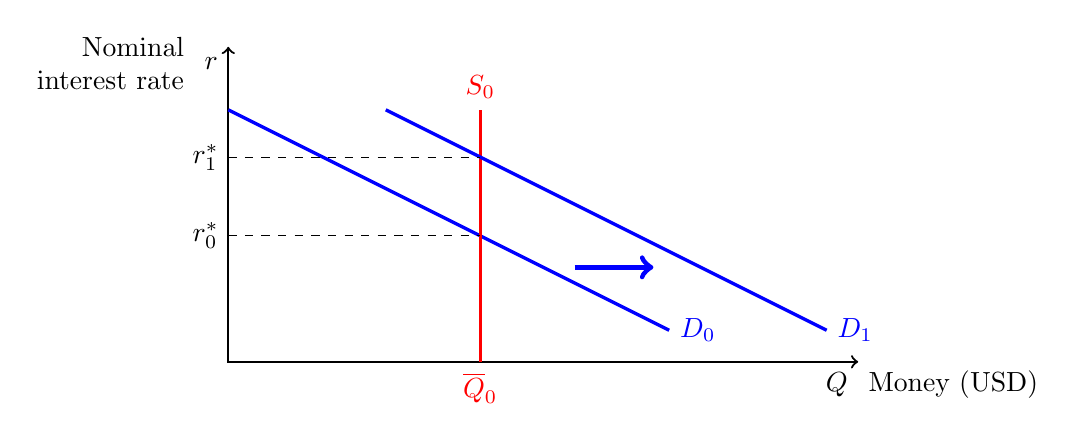
\begin{tikzpicture}[scale=0.4]
\draw[thick,<->] (0,10) node[below left,label={[align=right]left:Nominal\\interest rate}] {$r$} --(0,0)--(20,0) node[below left,label=right:Money (USD)]{$Q$};
\draw[very thick,blue] (0,8)--(14,1) node[right]{$D_0$};
\draw[very thick,red] (8,0) node[below]{$\overline{Q}_0$}--(8,8) node[above]{$S_0$};
\draw[dashed] (0,4) node[left]{$r^*_0$}--(8,4) node[right,yshift=4pt]{};
\draw[very thick, blue] (5,8)--(19,1) node[right]{$D_1$};
\draw[dashed] (0,6.5) node[left]{$r^*_1$}--(8,6.5) node[right,yshift=4pt]{};
\draw[line width=2pt,->,blue] (11,3)--(13.5,3);
\end{tikzpicture}

The market-clearing interest rate increases from $r^*_0$ to $r^*_1$. The quantity of money in circulation remains constant at $\overline{Q}_0$.
\end{solution}

\item Prior to this change in demand for the U.S.~dollar, the macroeconomy was in equilibrium at full employment. Using the model of aggregate demand and aggregate supply, please illustrate and explain the impact of the change in interest rates---from question 1, above---on GDP and the aggregate price level.

\begin{solution}
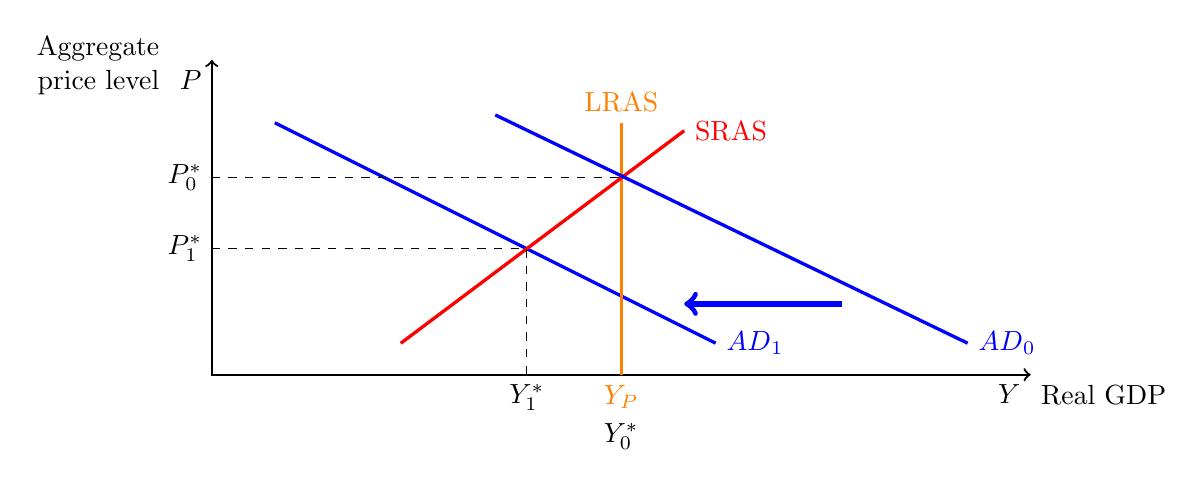
\begin{tikzpicture}[scale=0.4]
\draw[thick,<->] (0,10) node[below left,label={[align=right]left:Aggregate\\price level\\ }] {$P$} --(0,0)--(26,0) node[below left,label=right:Real GDP]{$Y$};
\draw[very thick,blue] (2,8)--(16,1) node[right]{$\text{AD}_1$};
\draw[very thick,orange] (13,0) node[below]{$Y_P$}--(13,8) node[above]{LRAS};
\draw[very thick,red] (6,1)--(15,7.75) node[right]{SRAS};
\draw[dashed] (0,4) node[left]{$P^*_1$}--(10,4) node[right,xshift=6pt]{} --(10,0)node[below]{$Y^*_1$};

\draw[very thick,blue] (9,8.25)--(24,1) node[right]{$\text{AD}_0$};
\draw[dashed] (0,6.25) node[left]{$P^*_0$}--(13,6.25) node[right,xshift=6pt]{};
\node[below,yshift=-14pt] at (13,0) {$Y^*_0$};

\draw[line width=2pt,->,blue] (20,2.25)--(15,2.25);
\end{tikzpicture}

The increase in the interest rate results in decreased consumer spending and decreased investment spending by firms, represented in this model by a decrease in aggregate demand (depicted here as shifting from $\text{AD}_0$ to $\text{AD}_1$). As a result, real output decreases from $Y^*_0$ to $Y^*_1$, while the aggregate price level decreases from $P^*_0$ to $P^*_1$.
\end{solution}

\item The Federal Reserve wants to \emph{exactly} reverse the impact of the change in interest rates on the macroeconomy.  What is one way in which the Fed can do this? Using the model of the money market illustrate the impact of such a policy on the nominal interest rate and the quantity of money.

\begin{solution}
The Federal Reserve has considerable influence over the money supply. If the Fed wants to reverse the impact of the interest rate change, it needs to increase money supply to reclaim $r^*_0$.\\

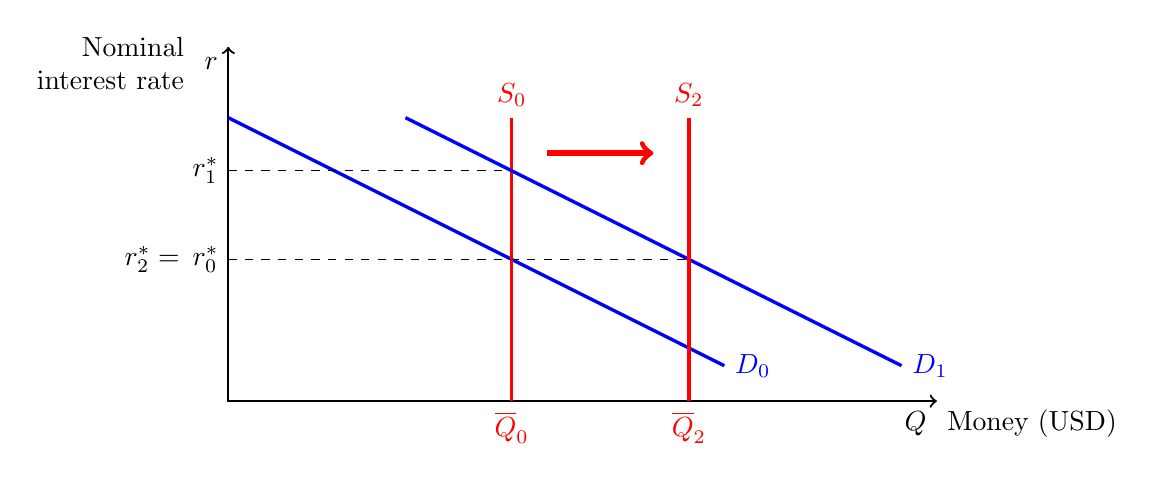
\begin{tikzpicture}[scale=0.45]
\draw[thick,<->] (0,10) node[below left,label={[align=right]left:Nominal\\interest rate}] {$r$} --(0,0)--(20,0) node[below left,label=right:Money (USD)]{$Q$};
\draw[very thick, blue] (0,8)--(14,1) node[right]{$D_0$};
\draw[very thick,red] (8,0) node[below]{$\overline{Q}_0$}--(8,8) node[above]{$S_0$};
\draw[dashed] (0,4) node[left]{$r^*_0$}--(8,4) node[right,yshift=8pt]{} --(13,4) node[right,yshift=4pt]{};
\draw[very thick, blue] (5,8)--(19,1) node[right]{$D_1$};
\draw[dashed] (0,6.5) node[left]{$r^*_1$}--(8,6.5) node[right,yshift=4pt]{};
\draw[very thick,red] (13,0) node[below]{$\overline{Q}_2$}--(13,8) node[above]{$S_2$};
\draw[line width=2pt,->,red] (9,7)--(12,7);
\draw(0,4) node[left,xshift=-14pt] {$r^*_2=$};
\end{tikzpicture}

To achieve $r^*_0$, the quantity of money in circulation must be increased to $\overline{Q}_2$ as depicted. This increase in the money supply lowers the interest rate from $r^*_1$ to $r^*_2$, where $r^*_2$ is equal to the intended goal of $r^*_0$.

To accomplish this, the Fed would likely use open market operations (OMO). To increase the money supply through OMO, the Federal Open Market Committee of the New York Federal Reserve would buy Treasury bonds. When the FOMC buys Treasury bonds, they inject money into the economy (the money used to buy the bonds) and remove the bonds from the economy.

The Fed could technically use two other monetary policy tools which are uncommon---adjustment of the reserve ratio or the discount rate. To increase money supply, the Fed would need to lower the reserve ratio or lower the discount rate. But as I've said in class, I want you to focus on OMO.
\end{solution}

\end{enumerate}

\end{document}
